\chapter{Svolgimento dello stage}
\label{cap:svolgimento}

\intro{Qui vengono raccolte tutte le principali attività svolte e osservazioni sul prodotto.}

\section{Analisi dei requisiti minimi del sistema}
\label{sez:requisiti}

Nei primi giorni in azienda era stato organizzato un'incontro formativo sul sistema di NDR da parte del fornitore, a cui mi è stato permesso di partecipare per seguire la presentazione di Sangfor. In questo incontro sono stati mostrati i vari strumenti che compongono il sistema di NDR e sono stati spiegati i concetti di base e casi d'uso. Vengono venduti in versione fisica \emph{on-premise} o virtualizzata, su cui è ricaduta la scelta di Wintech.

Dalle schede tecniche dei prodotti è possibile vedere le specifiche delle macchine e i requisiti minimi richiesti per la virtualizzazione. Questi sono stati raccolti rispettivamente in \autoref{tab:schede-tecniche} e \autoref{tab:requisiti-minimi}.

\begin{table}[!htbp]
    \centering
    \begin{tabularx}{\linewidth}{XX}
        \toprule
        \textbf{CyberCommand} & \textbf{Sonda STA} \\
        \midrule
        Memoria fino a 256GB di RAM & Fino a 32GB di RAM \\
        Fino a 20 core di CPU & Fino a 8 porte 10/100/1000 BaseT \\
        Supporto al RAID50 & Fino a 8 porte GBe SFP e fino a 4 porte 10GBe SFP+ \\
        Dimensioni fisiche: 2U & In versioni da 1U e 2U \\
            & Supporta fino a 12 interfacce di rete \\
        \bottomrule
    \end{tabularx}
    \caption{Scheda tecnica degli apparati fisici}
    \label{tab:schede-tecniche}
\end{table}

\begin{table}[!htbp]
    \centering
    \begin{tabularx}{\linewidth}{XX}
        \toprule
        \textbf{CyberCommand} & \textbf{Sonda STA} \\
        \midrule
        ISO basata su CentOS 7 & ISO basata su CentOS 7 \\
        Capacità di gestione fino a 7Gbps di traffico & Capacità di gestione fino a 2Gbps di traffico \\
        Supporta solo HCI o piattaforme certificate VMWare & Supporta solo piattaforme VMWare \\
        \bottomrule
    \end{tabularx}
    \caption{Requisiti minimi per le macchine virtuali}
    \label{tab:requisiti-minimi}
\end{table}

\section{Progettazione}

Al momento del mio arrivo in Wintech il sistema era stato appena installato e con una prima configurazione di base con una singola sonda, come \emph{Proof of Concept}. I primi giorni sono stati dedicati alla definizione delle configurazioni di un secondo NUC e del sistema di NDR, che è stato poi utilizzato per monitorare la rete interna dell'azienda.

Tutti i vari schemi di rete sono raccolti in \autoref{appendix:schemi}. Lo scopo di questi non è di essere una rappresentazione estremamente tecnica e dettagliata, ma più quello di dare un'idea generale e supporto grafico a quanto viene descritto testualmente. 

\subsection{Posizionamento delle sonde}

Durante il corso di presentazione del fornitore è stata presentata una possibile configurazione (\autoref{network:sangfor-sta-position}) di base per dove posizionare le sonde STA \cite{sangfor:product-slide}.

Come consigliato dal produttore, posizionarle tra i vari dispositivi permette loro di andare a monitorare anche traffico interno, riuscendo ad individuare i cosiddetti \emph{movimenti laterali} e possibili attacchi che non passano dall'esterno, come ad esempio l'espansione del controllo da parte di un \emph{malware} sui dispositivi.

In Wintech le varie sonde sono state dislocate una in sede, due tra i \emph{data center} e una da un cliente (schema in \autoref{network:wtc-sta-position})

\subsection{Configurazione dei dispositivi}

Come descritto nella \autoref{sez:requisiti} i dispositivi sono stati virtualizzati tramite l'\emph{hypervisor ESXi} di \emph{VMWare}. Questo prodotto era già conosciuto e in uso in Wintech, è stato solamente necessario adattare la configurazione per permettere alle sonde virtuali di funzionare correttamente avendo le interfacce di rete configurate per effettuare il \emph{mirroring} del traffico. Per fare questo sono stati utilizzati i \emph{commutatori virtuali} e i \emph{gruppi di porte}. Inoltre, per rendere i dispositivi tolleranti a perdita di corrente è stato configurato l'avvio automatico del sistema e delle macchine virtuali.

Un problema riscontrato con il \emph{software} di virtualizzazione è stata l'incompatibilità con gli \emph{E-Core} dei nuovi processori \emph{Intel} presenti nei NUC. Al momento l'unica soluzione è stata quella di disabilitarli, andando a sfruttare solo gli altri \emph{P-Core}, che sono comunque sufficienti per le esigenze del sistema.

\section{Controllo delle segnalazioni}

Uno dei punti chiave di uno strumento di questo tipo è quello di fornire segnalazioni utili all'amministratore per monitorare lo stato della rete. Durante tutto il periodo di stage il primo obiettivo è stato quello di capire quali fossero quelle più utili e come poterle sfruttare al meglio.

Ogni giorno una delle prime attività era proprio il controllo delle ultime segnalazioni, per capire se durante la notte ci fossero stati strani comportamenti nella rete. Dopo le prime settimane, dove sono state definite una serie di \emph{whitelist} per evitare falsi positivi, si è arrivati ad un sistema che segnalava solo i problemi più importanti e che richiedevano un controllo manuale da parte di un amministratore.

Principalmente sono stati esclusi tutti i problemi legati a sistemi in fase di test del \emph{team} di ricerca e sviluppo, le comunicazioni tra i \emph{software} di monitoraggio come PRTG e altri di \emph{backup}. Molto spesso \emph{scan} di rete effettuati in modalità automatica e generica da attaccanti che cercavano di trovare dispositivi vulnerabili portavano a segnalazioni di porte aperte note, ad esempio la 80 e la 443 per il sito \emph{web} aziendale.

\subsection{Segnalazioni di server security}

In generale le segnalazioni di \emph{Server Security} (\autoref{sec:cc-server-sec}) permettono di trovare anche problemi dovuti a configurazioni errate o a problemi di sicurezza non ancora risolti. In particolare, durante lo stage, sono state utili:

\begin{itemize}
    \item la funzione di rilevazione delle \emph{password} deboli, che è stata utilizzata definendo all'interno della lista di \emph{password} da segnalare alcune utilizzate in passato e che devono essere dismesse per motivi di sicurezza. In questo modo è stato possibile rilevare alcuni utenti che le utilizzavano ancora e che sono stati avvisati di cambiarle.
    \item tramite le segnalazioni \emph{Unencrypted Web Traffic} invece è stato possibile rilevare alcuni servizi di clienti in \emph{full-outsourcing} che non utilizzavano la versione sicura di HTTP. Questo ha permesso di avvisarli e di proporre loro una soluzione per risolvere il problema.
    \item la categoria \emph{Improper Configuration} che ha permesso di verificare se alcune configurazioni contengono errori noti o piccole dimenticanze che possono portare a problemi di sicurezza. Può tornare utile per rilevare situazioni in cui erano state aperte porte non standard per permettere l'accesso a servizi interni che non erano poi state chiuse dopo aver terminato il lavoro.
\end{itemize}

\subsection{Esempio di segnalazione: Infezione da \emph{Cryptominer} }
\label{sez:crypto-alert}

\begin{figure}[!htbp]
    \centering
    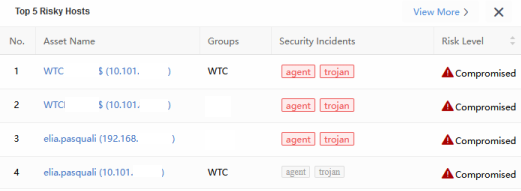
\includegraphics[width=0.8\linewidth]{images/ndr/crypto-host-sec.png}
    \caption{Segnalazioni di \emph{Cryptomining} in \emph{Host Security}}
    \label{fig:crypto-alerts}
\end{figure}

Nella \autoref{fig:crypto-alerts} possiamo vedere la situazione rilevata dal sistema NDR dopo che ho effettuato delle connessioni a siti legati a \emph{pool} di \emph{cryptomining}. Questo è stato fatto per testare il sistema e capire come funzionasse.

Dopo aver rilevato il traffico, ha segnalato l'host che ha effettuato le connessioni come compromesso, in quanto potenzialmente infetto da un \emph{miner} di criptovalute. Un difetto riscontrato nella segnalazione è che il mio dispositivo veniva rilevato più volte, in base a come questo si presentava sulla rete.

Discutendone con il tutor siamo arrivati alla conclusione che questo è legato alla struttura interna della rete Wintech e a come Windows gestisce le sue interfacce di rete e i nomi utente, che insieme al posizionamento consigliato per le sonde lo rende un problema di difficile risoluzione.

\subsection{Esempio di segnalazione: Richieste DNS malevole}

Un esempio che mostra come il sistema NDR analizza il traffico sono le segnalazioni legate a traffici DNS considerati malevoli. Durante il periodo di stage questa tipologia è stata oggetto di studio per capire come configurare al meglio il posizionamento del sistema e come definire una serie di \emph{whitelist} per evitare falsi positivi senza lasciare troppo traffico non controllato.

Le sonde, per loro natura e posizionamento interno alla rete, analizzano il traffico che passa "attraverso i cavi", rilevando quindi anche possibili attacchi che si proliferano tramite \emph{movimento laterale}. Questo porta ad avere segnalazioni di compromissione per ogni dispositivo in cui la richiesta DNS che il sistema ha catalogato come malevola transita.

Un piccolo diagramma qualitativo di questo processo è mostrato in \autoref{network:dns-multiple-request}, dove un dispositivo a dominio effettua una richiesta considerata malevola che passa per \emph{Domain Controller} e successivamente il \emph{firewall}.

\section{Test del prodotto}

Durante tutto il periodo di stage il sistema era attivo sulla rete e questo mi ha permesso di andare a testarlo in tutte le sue funzionalità e trovare i suoi limiti.

\subsection{Rilevazione di attacchi}

Tutti gli eventi malevoli scatenati per testare i tempi di risposta del sistema hanno mostrato che le rilevazioni sono quasi immediate, con ritardi dovuti solo al tempo di propagazione del traffico sulla rete. Una volta, dopo un'intensiva sessione di test che ha generato un'elevata dose di traffico, il sistema ha smesso di funzionare correttamente.

Questo problema è stato difficile da comprendere dato che la \emph{webapp} continuava ad essere attiva, semplicemente non era possibile interagire con i \emph{log}. Per prima cosa si è partiti con un'analisi diagnostica dello stato di salute del sistema, dal NUC alla macchina virtuale, che però non mostrava nessun problema. Dopo aver contattato il supporto, abbiamo scoperto che tutto ciò era dovuto ad un errore di configurazione della politica di rotazione dei \emph{log} e alla soglia critica impostata, che ha portato ad un blocco del disco virtuale.

La configurazione da correggere, essendo un parametro all'interno del \emph{database} del sistema, basato su \emph{ElasticSearch}, non era accessibile dall'interfaccia web, ma solo tramite \emph{SSH} e con credenziali non disponibili a noi. Dopo che il supporto ha corretto il problema, abbiamo provveduto ad aumentare lo spazio a disposizione della macchina, che era stato volutamente assegnato in quantità limitata per verificare se il requisito richiesto fosse effettivamente necessario e non fosse stato sovrastimato. Questa modifica ha rimesso in funzione il sistema e impedito al problema di ripresentarsi.

\subsection{Rilevazione di falle di sicurezza}

Come descritto nella \autoref{sec:cc-server-sec} il sistema è stato in grado di rilevare anche falle di sicurezza e configurazioni errate. Questo ha permesso di attivare i vari \emph{team} per occuparsi di questi problemi, passando da una prima analisi alla ricerca di soluzioni non invasive per il cliente, fino all'avviso di questi ultimi e alla proposta di soluzioni per risolvere i problemi.

\subsection{Rilevazione di \emph{malware}}

Spesso il sistema NDR si è rivelato attento ad ogni possibile strumento che operava in maniera malevola all'interno della rete. Sono stati utilizzati alcuni strumenti di \emph{crack} per le licenze di prodotti a pagamento per verificare la capacità di rilevazione di questo tipo di software. Bisogna considerare però che essendo un prodotto per la sicurezza della rete, non è in grado di rilevare software malevolo che lavora solamente in locale, ma solo se questo effettua connessioni verso l'esterno, per operazioni di \emph{command and control}, come nel caso esempio del \emph{cryptominer} (\autoref{sez:crypto-alert}).

\subsection{Usabilità}

Uno dei primi problemi riscontrati è stato quello di capire come utilizzare il sistema e come interpretare le segnalazioni. Per quanto l'interfaccia sia abbastanza intuitiva e rivolta ad un utenza con un minimo di bagaglio tecnico per comprendere ciò che viene mostrato, è comunque necessario un periodo di apprendimento per capire come utilizzare al meglio il sistema. Un fattore che ha rallentato alcune operazioni di configurazione è stata la documentazione non aggiornata o non completa. Questo ha portato a dover capire cosa alcune funzioni facessero tramite prove ed errori.

Molte volte le configurazioni potevano essere trovate sparse tra vari menù, inoltre spesso alcuni \emph{link} portavano senza preavviso ad altre pagine, che non essendo ben segnalate, erano difficili da raggiungere nuovamente successivamente. Molto spesso i parametri non avevano nomi parlanti, rendendo difficile comprendere il loro utilizzo. Questa situazione potrebbe essere dovuta allo sviluppo in Asia poi adattato per altri mercati, portando a delle traduzioni non sempre precise.

Nonostante tutto, questo problema è stato parzialmente limitato dall'estrema disponibilità del fornitore, che ha sempre cercato di risolvere i problemi e di fornire spiegazioni e chiarimenti, tramite scambi di email e sessioni di discussione e supporto remoto.

\section{Remediation}
\label{sec:remediation}

Una delle funzionalità più interessanti del sistema NDR è proprio quella di andare a risolvere autonomamente, dopo previa configurazione, alcuni problemi di sicurezza. Questo permette di avere un sistema che non solo rileva e segnala i problemi, ma che cerca anche di risolverli, permettendo di avere un sistema di sicurezza più completo e che richiede meno interventi manuali, evitando rallentamenti dovuti a tempi di risposta o assenza di operatori qualificati.

Come per le altre funzionalità, anche questa mancava di una documentazione adeguata, rendendo quindi necessaria una fase di studio e di test per capire come funzionasse e come poterla configurare al meglio. Dopo primi test basilari che andavano a lavorare internamente alla \emph{webapp} sul singolo dispositivo CyberCommand\cite{sangfor:policy-training} sono passato a testare l'integrazione con il sistema di \emph{Endpoint Protection} di \emph{Sangfor}\cite{sangfor:policy-edr-integration}.

\subsection{Esempio di remediation: scansione antivirus automatica}

Partiamo dalla definizione della policy, mostrata in \autoref{fig:policy-settings-trojan}

\begin{figure}[!htbp]
    \centering
    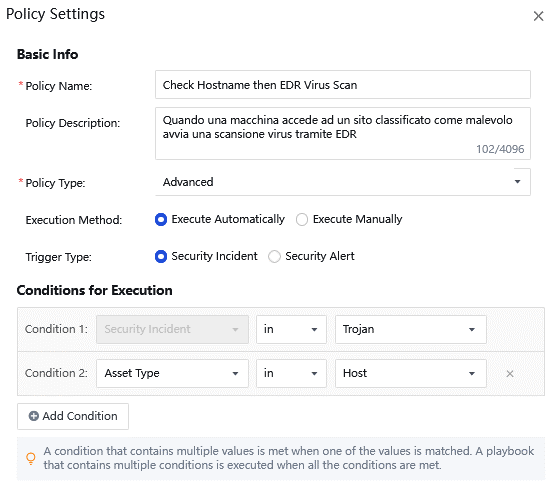
\includegraphics[scale=0.7]{images/ndr/policy-settings-trojan.png}
    \caption{Policy per la scansione antivirus automatica}
    \label{fig:policy-settings-trojan}
\end{figure}

Vediamo che è stata definita in modo da attivarsi quando viene rilevato un \emph{Incident} della categoria \emph{Trojan} e solo se il dispositivo interessato è un \emph{Host}, questo per escludere altri dispositivi di rete in cui richieste malevole transitano e non è possibile effettuare una scansione antivirus. La \emph{policy} è stata impostata per avviarsi in automatico.

\begin{figure}[!htbp]
    \centering
    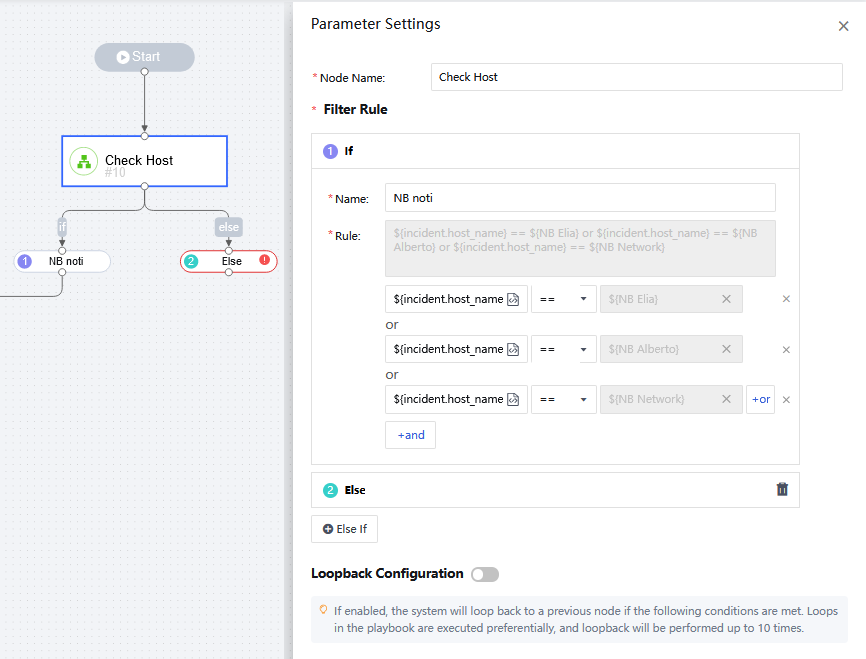
\includegraphics[width=0.8\linewidth]{images/ndr/decision-node-notebook.png}
    \caption{\emph{Decision node} per filtrare i dispositivi}
    \label{fig:notebook-filter}
\end{figure}

In \autoref{fig:notebook-filter} ho inserito un primo filtro per lavorare solamente su notebook che potevo "disturbare" durante i miei test, come il mio o quelli di altri stagisti. Questo è stato ottenuto tramite un \emph{decision node} che filtra i dispositivi in base al nome utente, che è stato impostato in fase di configurazione del sistema, salvati in una serie di costanti. Questo filtro è stato necessario per evitare di andare a disturbare i clienti con richieste di scansione antivirus.

Tutta la parte di effettiva attivazione della scansione si può vedere in \autoref{fig:scan-action-flow}. Tramite un \emph{action node} si avvia sul programma \emph{EDR} installato sul dispositivo una scansione di tipo \emph{Full Scan} (\autoref{fig:scan-action-node}). Successivamente si è aggiunto un \emph{decision node} che controlla se la scansione è terminata con successo o meno, sfruttando il sistema di \emph{loopback} per ricontrollarne lo stato fino alla terminazione, con successo o meno.

\begin{figure}[!htbp]
    \centering
    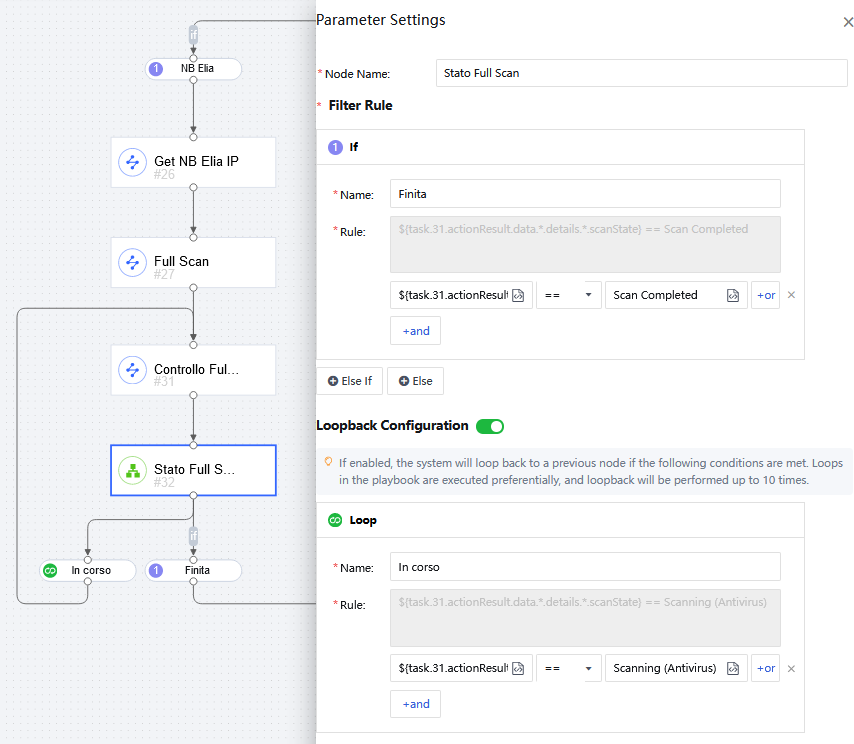
\includegraphics[width=0.9\linewidth]{images/ndr/scan-action-flow.png}
    \caption{Configurazione della scansione}
    \label{fig:scan-action-flow}
\end{figure}

\begin{figure}[!htbp]
    \centering
    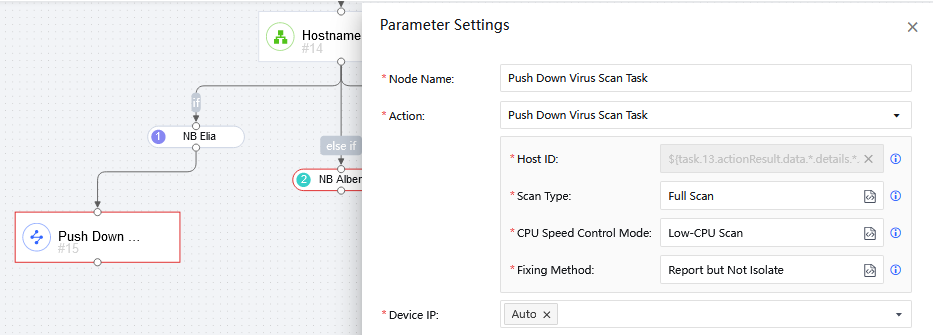
\includegraphics[width=0.9\linewidth]{images/ndr/scan-action-node.png}
    \caption{\emph{Action node} per avviare la scansione}
    \label{fig:scan-action-node}
\end{figure}

\subsection{Problemi riscontrati}

Durante la configurazione di questa funzionalità sono stati riscontrati diversi problemi, alcuni dei quali sono stati risolti tramite l'assistenza del fornitore, altri invece sono ancora presenti.

\subsubsection{Problemi nella gestione dei parametri multipli}

Il sistema permette di definire regole con parametri multipli, divisi da virgole. In caso di parametri predefiniti o costanti, che vengono salvati come stringhe e poi recuperati tramite la sintassi \texttt{\$nome\_parametro}, viene mostrato un errore e limitato ad un singolo simbolo \texttt{\$}, come mostrato in \autoref{fig:single-dollar}

\begin{figure}[!htbp]
    \centering
    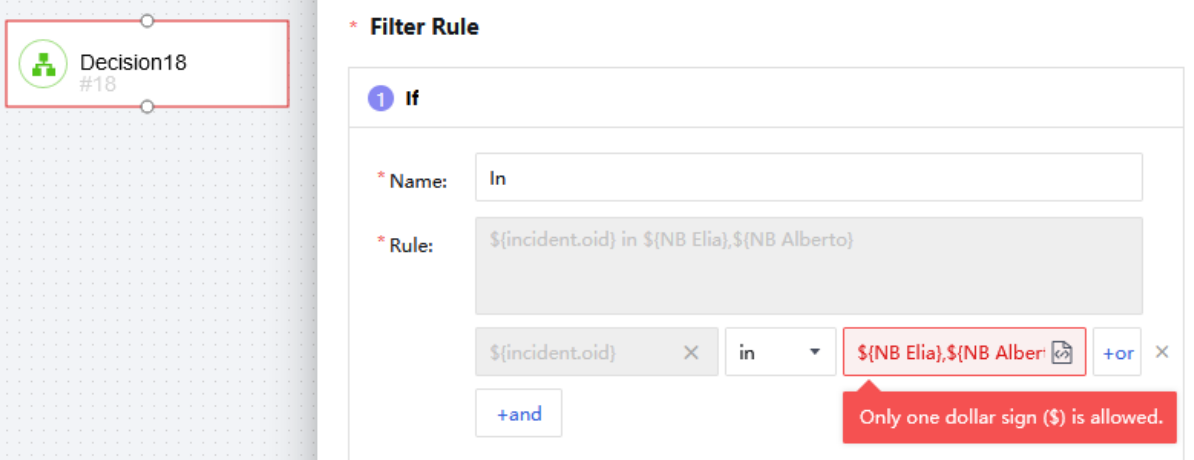
\includegraphics[width=0.9\linewidth]{images/ndr/single-dollar.png}
    \caption{Errore nella gestione dei parametri multipli}
    \label{fig:single-dollar}
\end{figure}

\subsubsection{Mancanza di documentazione}

Per prima cosa, come già accennato, la documentazione non era completa e non era possibile capire come funzionasse la funzionalità senza fare dei test. Dopo aver fatto delle ricerche sul forum della community\cite{forum:sangfor-community} di \emph{Sangfor} ho trovato un post che accennava a dei documenti, che però non erano disponibili. Dopo aver contattato il \emph{team} italiano, mi è stato fornito un documento con la raccolta dei parametri disponibili per la configurazione delle \emph{policy}, anche se non era ancora completo\cite{sangfor:policy-parameter}.

\subsubsection{Mancanza di feedback sullo stato della scansione}

Per ottenere un feedback sullo stato delle azioni era necessario andare a controllare i \emph{log} in una sezione non facilmente raggiungibile. Questi però si limitavano a mostrare se l'azione aveva completato con successo o meno, con piccole informazioni sugli errori, come mostrato in \autoref{fig:failed-response}. Questo ha portato a dover fare diversi test per capire come funzionasse la funzionalità e come poterla configurare al meglio.

\begin{figure}[!htbp]
    \centering
    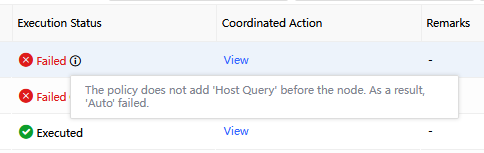
\includegraphics[width=0.9\linewidth]{images/ndr/failed-response.png}
    \caption{Esempio di \emph{log} di errore}
    \label{fig:failed-response}
\end{figure}

\subsubsection{Mancanza di un sistema di test}

Un altro problema riscontrato è stato quello di non avere un sistema di test per verificare il funzionamento delle \emph{policy} prima di applicarle. Questo ha portato a dover fare diversi test scatenando falsi positivi, rallentando la configurazione delle risposte.

\subsubsection{Limitazioni nelle integrazioni}

Questo problema è legato al fatto che il prodotto è ancora nuovo. Per offrire l'integrazione con strumenti di terze parti è necessario per il \emph{team} di sviluppo di \emph{Sangfor} ottenere un'interfaccia di programmazione (\emph{API}) da parte dei competitor. Dopo un dialogo con il \emph{team} italiano ci è stato detto che tutto questo è attualmente una delle priorità del produttore.

\subsubsection{Definizione delle policy macchinosa}
\label{sez:policy-macchinosa}

La definizione di \emph{policy} tramite questo strumento grafico riesce ad essere intuitivo e va a limitare la mancanza di documentazione su come produrre queste regole. Forse a causa della mia formazione informatica, ho trovato che la definizione di queste regole fosse macchinosa e sarebbe stata estremamente più chiara e manutenibile se fosse stata definibile tramite uno strumento testuale, come ad esempio un linguaggio di \emph{scripting}.

Tramite regole testuali sarebbe stato possibile anche definire delle \emph{policy} tramite un sistema di \emph{template}, che avrebbe permesso di velocizzare la configurazione e di avere un sistema di test più semplice. Inoltre, si sarebbe potuto sfruttare un sistema di versionamento come \emph{Git}, per tenere traccia delle modifiche apportate e per poter effettuare \emph{rollback} in caso di problemi.

\section{Report tramite API REST}

Le funzionalità di creazione di \emph{report} offerte dal sistema si limitavano alla produzione di \emph{file} PDF con un consuntivo sull'andamento e lo stato della rete rispetto ad un particolare periodo. Utilizzando lo strumento però si sentiva la necessità di estrarre dei dati in formati strutturati come \emph{JSON} o \emph{CSV} per poterli utilizzare in altri strumenti, ad esempio integrandoli agli altri sistemi di monitoraggio o creando delle \emph{dashboard} personalizzate con lo stack ELK, ovvero \emph{Logstash} per processare i dati, \emph{ElasticSearch} per l'indicizzazione e \emph{Kibana} per la visualizzazione.

\subsection{Problemi riscontrati}

Il primo problema riscontrato è stato quello di capire come funzionasse il sistema di autenticazione per le API. Dopo aver fatto delle ricerche sul forum della community\cite{forum:sangfor-community} di \emph{Sangfor} ho trovato un \emph{post} che conteneva al suo interno un documento\cite{sangfor:rest-api}, che sembrava essere abbastanza recente. 

Dopo alcune prove, che non hanno portato ad alcun risultato, ho contattato il \emph{team} di supporto, che mi ha confermato che il documento si riferiva ad una versione precedente del sistema, che non era più valido e che non era disponibile una documentazione aggiornata, dato che era in programma un aggiornamento importante del sistema con una probabile riscrittura di queste funzionalità. 

\subsection{Soluzione alternativa}

Per ottenere dei dati dall'NDR in un formato utile al mio scopo ho cercato di estrarli dalle richieste che vengono effettuate normalmente dalla \emph{webapp}, analizzandole tramite gli strumenti da sviluppatore integrati nei \emph{browser}. Questa via non ha portato a risultati soddisfacenti, quindi sono passato ad una tecnica più invasiva, tramite del \emph{web scraping} con \emph{Python}, sfruttando la libreria \emph{Selenium} e \emph{requests} per estrarre i dati dalle pagine.

Nonostante questo, la soluzione è risultata essere molto macchinosa e poco performante, in quanto richiedeva di simulare l'accesso alla \emph{webapp} e di navigare tra le varie pagine per estrarre i dati. Inoltre, il sistema di autenticazione tramite \emph{token} ha portato a dover aggiornare manualmente il codice ogni volta che questo cambiava, rendendo la soluzione poco manutenibile.